\documentclass[border=2pt]{standalone}
\usepackage{tikz}
\usetikzlibrary{arrows.meta,chains,%
                    decorations.pathreplacing}
\usetikzlibrary{matrix,positioning,arrows.meta,arrows}

\tikzset{
mymat/.style={
  matrix of nodes,
  nodes in empty cells,
  text height=2.5ex,
  text depth=0.75ex,
  text width=3.25ex,
  align=center,
  column sep=-\pgflinewidth
  }
}
\tikzset{
  rows/.style 2 args={
    sub@rows/.style={row ##1 column #2/.style={nodes={rectangle,draw=black}}},
    sub@rows/.list={#1}
  },
  box/.style 2 args={
    sub@box/.style={rows={#1}{##1}},
    sub@box/.list={#2}
  }
}
\begin{document}

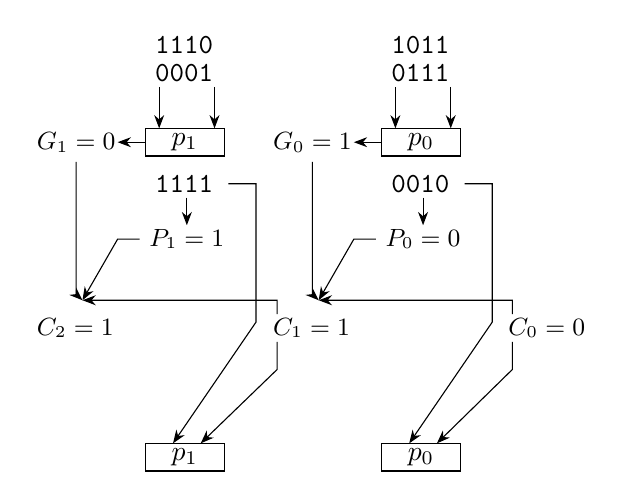
\begin{tikzpicture}[>=latex]

%% stage 1
\coordinate(A1) at(0, 0);
\coordinate(A0) at(3, 0);
\coordinate(B1) at(0, -5);
\coordinate(B0) at(3, -5);
\coordinate(D1) at(0, -4);
\coordinate(D0) at(3, -4);
\coordinate[below left=0em and 0cm of A1](In1-1);
\coordinate[below left=1em and 0cm of A1](In1-2);
\coordinate[below left=4em and 0cm of A1](Adder1);
\coordinate[below left=5em and 0cm of A1](Out1-1);

\node[anchor=west] at(In1-1) {$\texttt{1110}$};
\node[anchor=west] at(In1-2) {$\texttt{0001}$};
\node[anchor=west] at(Out1-1) {$\texttt{1111}$};

\draw (Adder1) rectangle +(1, 1em) node[pos=.5] {$p_1$};


\draw[-{Stealth[scale=1.0]}] ([xshift=0.5em,yshift=-0.5em]In1-2) -- ([xshift=0.5em,yshift=1em]Adder1);
\draw[-{Stealth[scale=1.0]}] ([xshift=2.5em,yshift=-0.5em]In1-2) -- ([xshift=2.5em,yshift=1em]Adder1);

\draw[-{Stealth[scale=1.0]}] ([xshift=0em,yshift=0.5em]Adder1) -- ([xshift=-1.0em,yshift=0.5em]Adder1) node[pos=2.5](G1) {\small $G_1 = 0$};

\draw[-{Stealth[scale=1.0]}] ([xshift=1.5em,yshift=-1.5em]Adder1) -- ([xshift=1.5em,yshift=-2.5em]Adder1) node[pos=1.5](P1) {\small $P_1 = 1$};

%%

\coordinate[below left=0em and 0cm of A0](In2-1);
\coordinate[below left=1em and 0cm of A0](In2-2);
\coordinate[below left=4em and 0cm of A0](Adder2);
\coordinate[below left=5em and 0cm of A0](Out2-1);

\node[anchor=west] at(In2-1) {$\texttt{1011}$};
\node[anchor=west] at(In2-2) {$\texttt{0111}$};
\node[anchor=west] at(Out2-1) {$\texttt{0010}$};

\draw (Adder2) rectangle +(1, 1em) node[pos=.5] {$p_0$};


\draw[-{Stealth[scale=1.0]}] ([xshift=0.5em,yshift=-0.5em]In2-2) -- ([xshift=0.5em,yshift=1em]Adder2);
\draw[-{Stealth[scale=1.0]}] ([xshift=2.5em,yshift=-0.5em]In2-2) -- ([xshift=2.5em,yshift=1em]Adder2);

\draw[-{Stealth[scale=1.0]}] ([xshift=0em,yshift=0.5em]Adder2) -- ([xshift=-1.0em,yshift=0.5em]Adder2) node[pos=2.5](G0) {\small $G_0 = 1$};

\draw[-{Stealth[scale=1.0]}] ([xshift=1.5em,yshift=-1.5em]Adder2) -- ([xshift=1.5em,yshift=-2.5em]Adder2) node[pos=1.5](P0) {\small $P_0 = 0$};

%%

\coordinate[below left=6em and 0cm of G0](C1);
\coordinate[below left=6em and 0cm of G1](C2);
\coordinate[left=-8.5em of C1](C0);

\node[anchor=west] at(C0) {\small $C_0 = 0$};
\node[anchor=west] at(C1) {\small $C_1 = 1$};
\node[anchor=west] at(C2) {\small $C_2 = 1$};

%% decider C

\draw[-{Stealth[scale=1.0]}] ([xshift=0.5em,yshift=0.5em]C1) -- +(0,0.5em) -- ([xshift=2em,yshift=1em]C2);
\draw[-{Stealth[scale=1.0]}] ([xshift=-1em,yshift=-0.5em]G1) -- +(1em,-5em) -- ([xshift=2em,yshift=1em]C2);
\draw[-{Stealth[scale=1.0]}] ([xshift=0.5em,yshift=1em]P1) -- +(-3em,-1em) -- ([xshift=2em,yshift=1em]C2);

\draw[-{Stealth[scale=1.0]}] ([xshift=0.5em,yshift=0.5em]C0) -- +(0,0.5em) -- ([xshift=2em,yshift=1em]C1);
\draw[-{Stealth[scale=1.0]}] ([xshift=-1em,yshift=-0.5em]G0) -- +(1em,-5em) -- ([xshift=2em,yshift=1em]C1);
\draw[-{Stealth[scale=1.0]}] ([xshift=0.5em,yshift=1em]P0) -- +(-3em,-1em) -- ([xshift=2em,yshift=1em]C1);

%% stage 2

\coordinate[below left=0em and 0cm of D1](In3-1);
\coordinate[below left=1em and 0cm of D1](In3-2);
\coordinate[below left=4em and 0cm of D1](Adder3);
\coordinate[below left=5em and 0cm of D1](Out3-1);

\draw (Adder3) rectangle +(1, 1em) node[pos=.5] {$p_1$};

\draw[-{Stealth[scale=1.0]}] ([xshift=0.5em,yshift=-0.5em]C1) -- +(0,-1em) -- ([xshift=2em,yshift=1em]Adder3);
\draw[-{Stealth[scale=1.0]}] ([xshift=3em,yshift=0em]Out1-1) -- +(1em, 0em) -- +(1em,-5em) -- ([xshift=1em,yshift=1em]Adder3);

\coordinate[below left=0em and 0cm of D0](In4-1);
\coordinate[below left=1em and 0cm of D0](In4-2);
\coordinate[below left=4em and 0cm of D0](Adder4);
\coordinate[below left=5em and 0cm of D0](Out4-1);

\draw (Adder4) rectangle +(1, 1em) node[pos=.5] {$p_0$};

\draw[-{Stealth[scale=1.0]}] ([xshift=0.5em,yshift=-0.5em]C0) -- +(0,-1em) -- ([xshift=2em,yshift=1em]Adder4);
\draw[-{Stealth[scale=1.0]}] ([xshift=3em,yshift=0em]Out2-1) -- +(1em, 0em) -- +(1em,-5em) -- ([xshift=1em,yshift=1em]Adder4);

\end{tikzpicture}

\end{document}